\section{Top Class Reference}
\label{classTop}\index{Top@{Top}}
{\tt \#include $<$top.h$>$}

Inheritance diagram for Top:\begin{figure}[H]
\begin{center}
\leavevmode
\includegraphics[width=88pt]{classTop__inherit__graph}
\end{center}
\end{figure}
Collaboration diagram for Top:\begin{figure}[H]
\begin{center}
\leavevmode
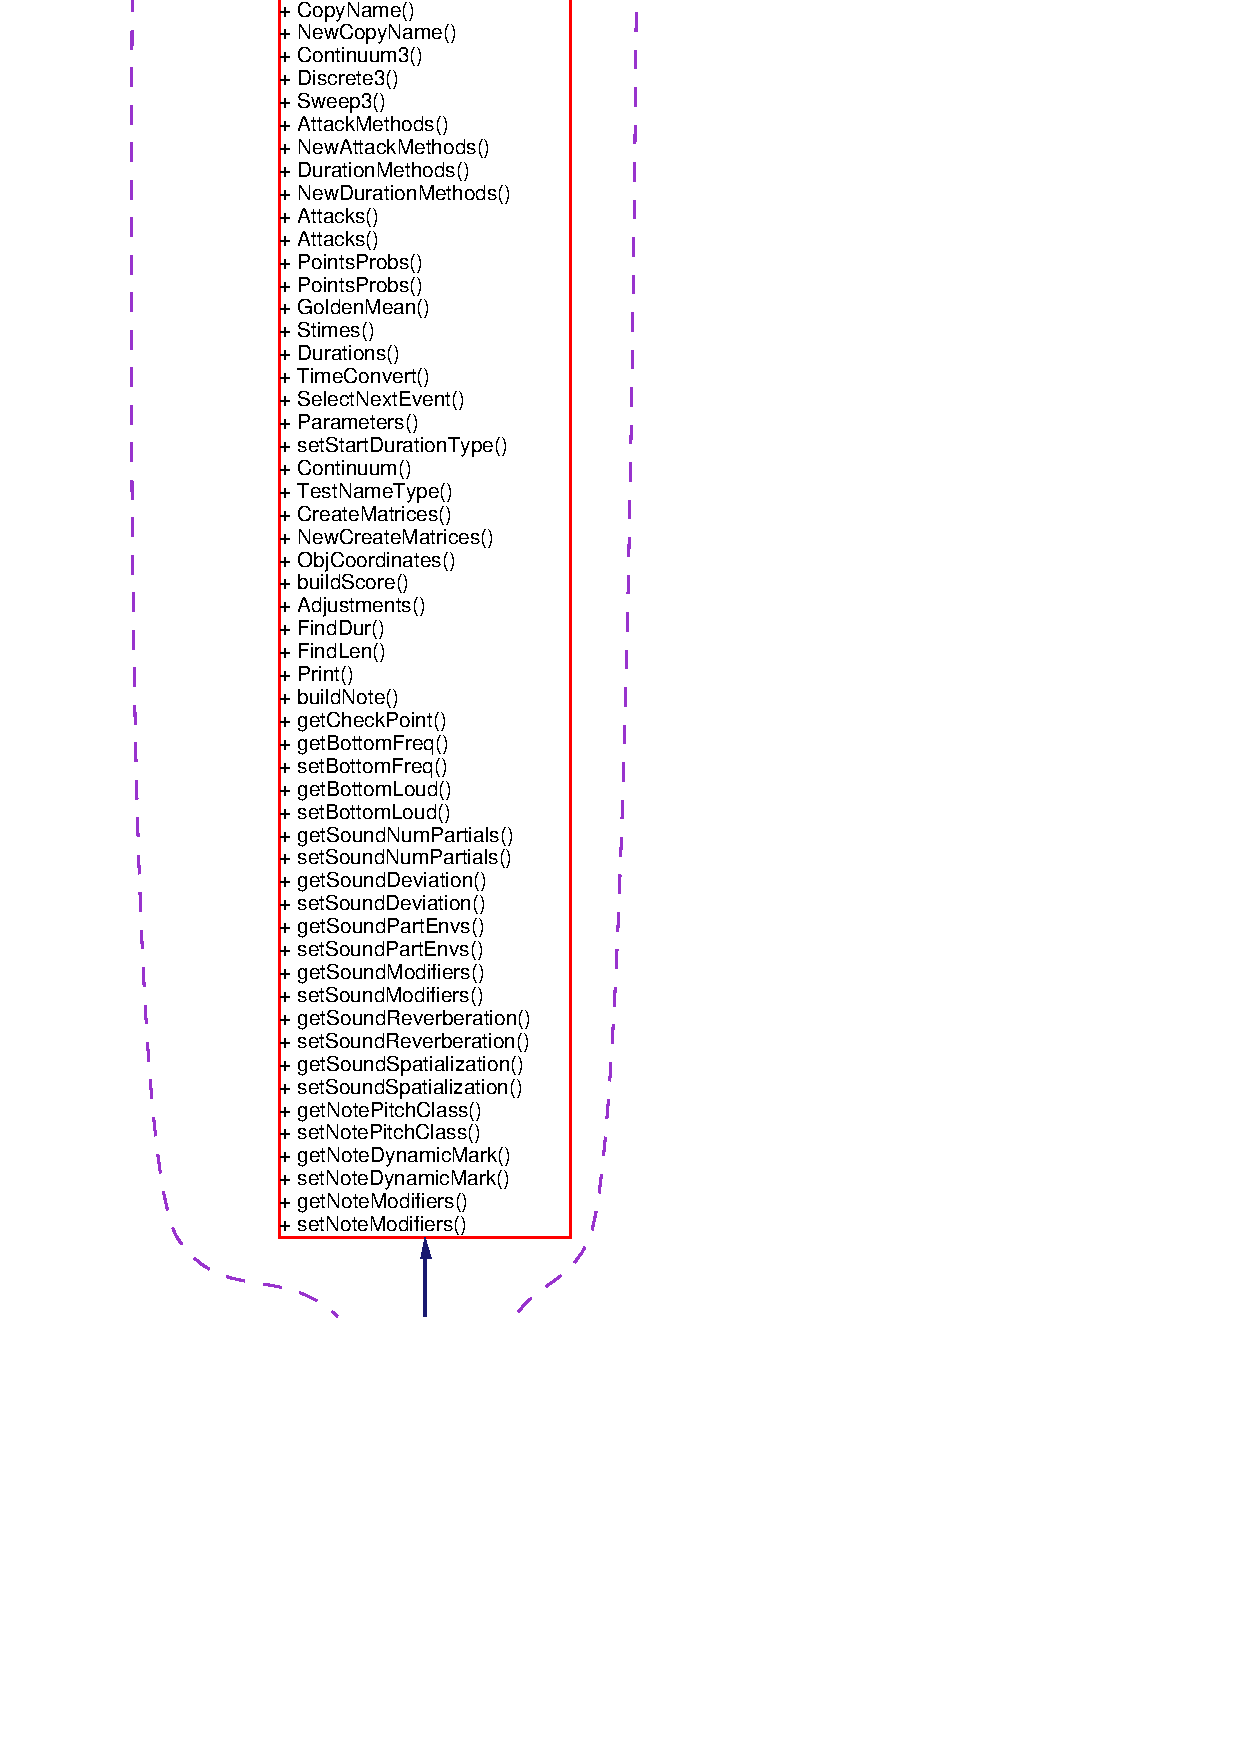
\includegraphics[width=186pt]{classTop__coll__graph}
\end{center}
\end{figure}
\subsection*{Public Member Functions}
\begin{CompactItemize}
\item 
{\bf Top} (char $\ast${\bf a\-Name})
\item 
{\bf Top} (float a\-Start\-Time, float a\-Duration, int a\-Type, char $\ast${\bf a\-Name})
\item 
{\bf Top} (const  {\bf Top} \&orig\-Top)
\item 
{\bf $\sim$Top} ()
\item 
void {\bf clear} ()
\item 
virtual void {\bf set\-Start\-Time} (float a\-Start\-Time)
\item 
virtual void {\bf Set\-Duration} (float a\-Duration)
\item 
float {\bf Set\-Dens} (double a\-Density)
\item 
void {\bf Print} ()
\end{CompactItemize}
\subsection*{Private Member Functions}
\begin{CompactItemize}
\item 
int {\bf Stimes} ()
\end{CompactItemize}
\subsection*{Private Attributes}
\begin{CompactItemize}
\item 
char $\ast$ {\bf file\-Name}
\item 
int {\bf levels}
\item 
int {\bf length}
\end{CompactItemize}


\subsection{Constructor \& Destructor Documentation}
\index{Top@{Top}!Top@{Top}}
\index{Top@{Top}!Top@{Top}}
\subsubsection{\setlength{\rightskip}{0pt plus 5cm}Top::Top (char $\ast$ {\em a\-Name})}\label{classTop_a0}


CONSTRUCTOR: Top. Empty, generic event; has only a name. 

Definition at line 48 of file top.cpp.

References Event::a\-Name, Event::keep\-Name, Event::obj\-ID, and Event::set\-Name().

Here is the call graph for this function:\begin{figure}[H]
\begin{center}
\leavevmode
\includegraphics[width=113pt]{classTop_a0_cgraph}
\end{center}
\end{figure}
\index{Top@{Top}!Top@{Top}}
\index{Top@{Top}!Top@{Top}}
\subsubsection{\setlength{\rightskip}{0pt plus 5cm}Top::Top (float {\em a\-Start\-Time}, float {\em a\-Duration}, int {\em a\-Type}, char $\ast$ {\em a\-Name})}\label{classTop_a1}


CONSTRUCTOR: Top (All fundamental information) 

Definition at line 61 of file top.cpp.

References Event::a\-Name, Event::keep\-Name, Event::set\-Duration(), Event::set\-Name(), and set\-Start\-Time().

Here is the call graph for this function:\begin{figure}[H]
\begin{center}
\leavevmode
\includegraphics[width=120pt]{classTop_a1_cgraph}
\end{center}
\end{figure}
\index{Top@{Top}!Top@{Top}}
\index{Top@{Top}!Top@{Top}}
\subsubsection{\setlength{\rightskip}{0pt plus 5cm}Top::Top (const {\bf Top} \& {\em orig\-Top})}\label{classTop_a2}


CONSTRUCTOR: Top (copy constructor) 

Definition at line 75 of file top.cpp.\index{Top@{Top}!~Top@{$\sim$Top}}
\index{~Top@{$\sim$Top}!Top@{Top}}
\subsubsection{\setlength{\rightskip}{0pt plus 5cm}Top::$\sim${\bf Top} ()}\label{classTop_a3}


DESTRUCTOR: $\sim$Top 

Definition at line 85 of file top.cpp.

\subsection{Member Function Documentation}
\index{Top@{Top}!clear@{clear}}
\index{clear@{clear}!Top@{Top}}
\subsubsection{\setlength{\rightskip}{0pt plus 5cm}void Top::clear ()\hspace{0.3cm}{\tt  [virtual]}}\label{classTop_a4}


Clears several internal structures in the {\bf Event}{\rm (p.\,\pageref{classEvent})}: name\-Type, max\-Types, layer\-Dens, objs\-In\-Layer, remain\-Objs, types\-In\-Layer, star\-Tarray, prob\-Sieve\-Array, dur\-Array, prob\-Dur\-Array 

Reimplemented from {\bf Event} {\rm (p.\,\pageref{classEvent_a12})}.

Definition at line 93 of file top.cpp.\index{Top@{Top}!Print@{Print}}
\index{Print@{Print}!Top@{Top}}
\subsubsection{\setlength{\rightskip}{0pt plus 5cm}void Top::Print ()\hspace{0.3cm}{\tt  [virtual]}}\label{classTop_a8}


Print 

Reimplemented from {\bf Event} {\rm (p.\,\pageref{classEvent_a57})}.

Definition at line 136 of file top.cpp.

References output\-File, Event::the\-Duration, Event::the\-Name, Event::the\-Start\-Time, and Event::u\-Per\-Sec.\index{Top@{Top}!SetDens@{SetDens}}
\index{SetDens@{SetDens}!Top@{Top}}
\subsubsection{\setlength{\rightskip}{0pt plus 5cm}float Top::Set\-Dens (double {\em a\-Density})}\label{classTop_a7}


Set the density of the top level 

Definition at line 107 of file top.cpp.

References Event::the\-Density.\index{Top@{Top}!SetDuration@{SetDuration}}
\index{SetDuration@{SetDuration}!Top@{Top}}
\subsubsection{\setlength{\rightskip}{0pt plus 5cm}void Top::Set\-Duration (float {\em a\-Duration})\hspace{0.3cm}{\tt  [virtual]}}\label{classTop_a6}


Set\-Duration 

Definition at line 126 of file top.cpp.

References Event::the\-Duration.\index{Top@{Top}!setStartTime@{setStartTime}}
\index{setStartTime@{setStartTime}!Top@{Top}}
\subsubsection{\setlength{\rightskip}{0pt plus 5cm}void Top::set\-Start\-Time (float {\em a\-Start\-Time})\hspace{0.3cm}{\tt  [virtual]}}\label{classTop_a5}


Set\-Start\-Time 

Reimplemented from {\bf Event} {\rm (p.\,\pageref{classEvent_a7})}.

Definition at line 117 of file top.cpp.

References Event::the\-Start\-Time.

Referenced by Top().\index{Top@{Top}!Stimes@{Stimes}}
\index{Stimes@{Stimes}!Top@{Top}}
\subsubsection{\setlength{\rightskip}{0pt plus 5cm}int Top::Stimes ()\hspace{0.3cm}{\tt  [private]}}\label{classTop_d0}


\begin{Desc}
\item[{\bf Deprecated}]DO NOT USE (Used to be private... not sure why it isn't anymore) \end{Desc}


Reimplemented from {\bf Event} {\rm (p.\,\pageref{classEvent_a42})}.

\subsection{Member Data Documentation}
\index{Top@{Top}!fileName@{fileName}}
\index{fileName@{fileName}!Top@{Top}}
\subsubsection{\setlength{\rightskip}{0pt plus 5cm}char$\ast$ {\bf Top::file\-Name}\hspace{0.3cm}{\tt  [private]}}\label{classTop_r0}




Definition at line 65 of file top.h.\index{Top@{Top}!length@{length}}
\index{length@{length}!Top@{Top}}
\subsubsection{\setlength{\rightskip}{0pt plus 5cm}int {\bf Top::length}\hspace{0.3cm}{\tt  [private]}}\label{classTop_r2}




Reimplemented from {\bf Event} {\rm (p.\,\pageref{classEvent_o20})}.

Definition at line 66 of file top.h.\index{Top@{Top}!levels@{levels}}
\index{levels@{levels}!Top@{Top}}
\subsubsection{\setlength{\rightskip}{0pt plus 5cm}int {\bf Top::levels}\hspace{0.3cm}{\tt  [private]}}\label{classTop_r1}




Reimplemented from {\bf Event} {\rm (p.\,\pageref{classEvent_o19})}.

Definition at line 66 of file top.h.

The documentation for this class was generated from the following files:\begin{CompactItemize}
\item 
{\bf top.h}\item 
{\bf top.cpp}\end{CompactItemize}
